\section{Experiments}
\label{sec:exp}

SECDO does not target Pareto dominance on all metrics.
We evaluate (i)~scaling structure on synthetic convex problems, (ii)~optimality--safety trade-off on UAV allocation, and (iii)~prediction-failure stress tests.

\subsection{Experimental Setup}
\textbf{Synthetic convex:} theory validation of Theorem~\ref{thm:2} scaling and PI behavior---not leaderboard tuning.
\textbf{UAV system evaluation:} practical benefit and safety/efficiency trade-off under Slow/Fast/Stress regimes (5 seeds); this demonstrates system behavior only (synthetic experiments address scaling laws).
\textbf{Prediction failure stress test:} Corollary~\ref{cor:4} via corrupted $\hat c$ windows.

\subsection{Dynamic Regret Scaling}
\begin{figure}[t]
\centering
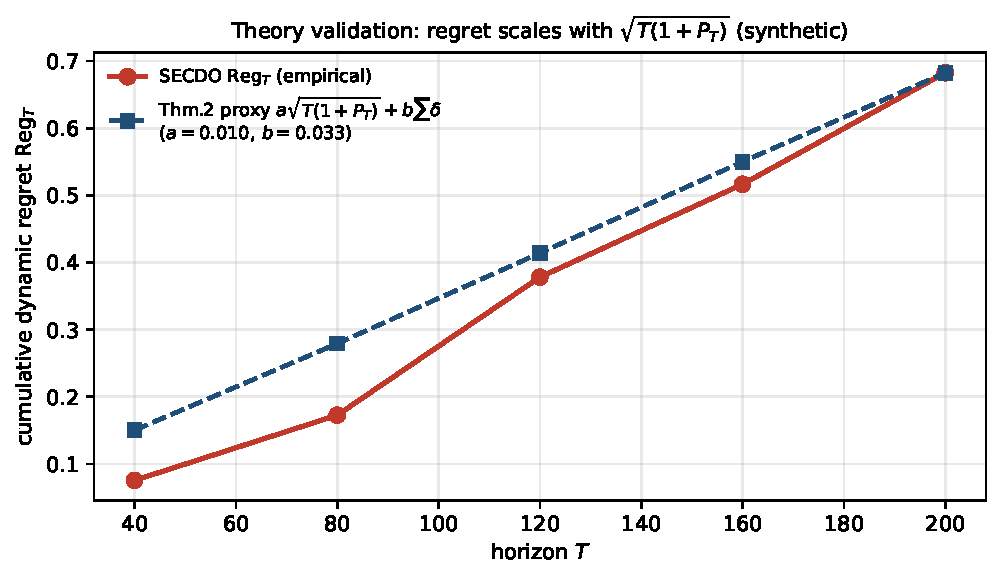
\includegraphics[width=\linewidth]{figures/fig4_regret.pdf}
\caption{Dynamic regret scaling under synthetic evolving constraints.
Empirical $\mathrm{Reg}_T$ tracks the structure $O\sqrt{T(1+P_T)}+O\sum\delta$.
The fitted envelope is only used for visualization and does not represent a universal constant.}
\label{fig:regret}
\end{figure}

Fig.~\ref{fig:regret} demonstrates the \emph{scaling behavior} predicted by Theorem~\ref{thm:2}.
Coefficients in the plotted envelope are fitted only for visualization.

\subsection{Drift Sensitivity on UAV}
\begin{table}[t]
\centering
\caption{SECDO under increasing environmental drift (5 seeds).}
\label{tab:drift}
\begin{tabular}{lccc}
\toprule
Regime & $\bar\chi$ & $\mathrm{Reg}_T$ & Violation \\
\midrule
Slow   & 0.010 & $7.69\times10^{-4}$ & 0.33\% \\
Fast   & 0.131 ($\times$13.0) & $4.36\times10^{-2}$ ($\times$56.7) & 1.46\% \\
Stress & 0.203 & $6.86\times10^{-2}$ & 1.89\% \\
\bottomrule
\end{tabular}
\end{table}
Table~\ref{tab:drift}: a $13\times$ rise in $\bar\chi$ induces a $56.7\times$ rise in $\mathrm{Reg}_T$ with bounded violation.

\subsection{Failure Recovery and PI Adaptation}
\begin{figure}[t]
\centering
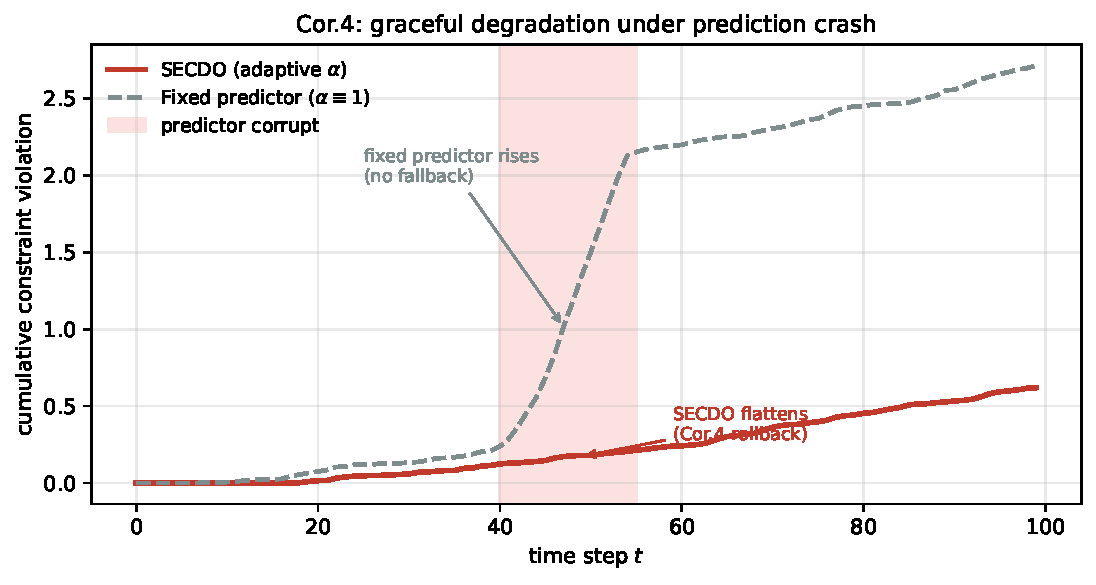
\includegraphics[width=\linewidth]{figures/fig2_crash.pdf}
\caption{Robust recovery under predictor failure (crash protocol).
SECDO gracefully degrades relative to fixed $\alpha\equiv 1$.}
\label{fig:crash}
\end{figure}
\begin{figure}[t]
\centering
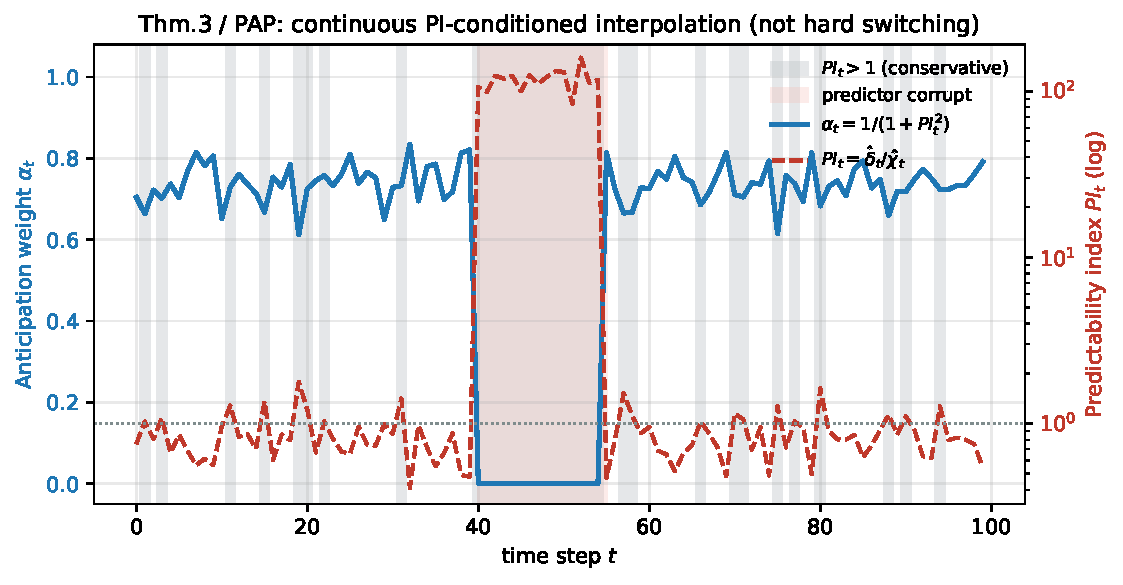
\includegraphics[width=\linewidth]{figures/fig3_PI_boundary.pdf}
\caption{Online $\mathrm{PI}_t$ and adaptive weight $\alpha_t=1/(1+\mathrm{PI}_t^2)$ under predictor corruption.}
\label{fig:pi}
\end{figure}
Figs.~\ref{fig:crash}--\ref{fig:pi} demonstrate the empirical behavior predicted by Corollary~\ref{cor:4}
and predictability-conditioned mixing.

\subsection{Optimality--Safety Trade-off}
\begin{figure}[t]
\centering
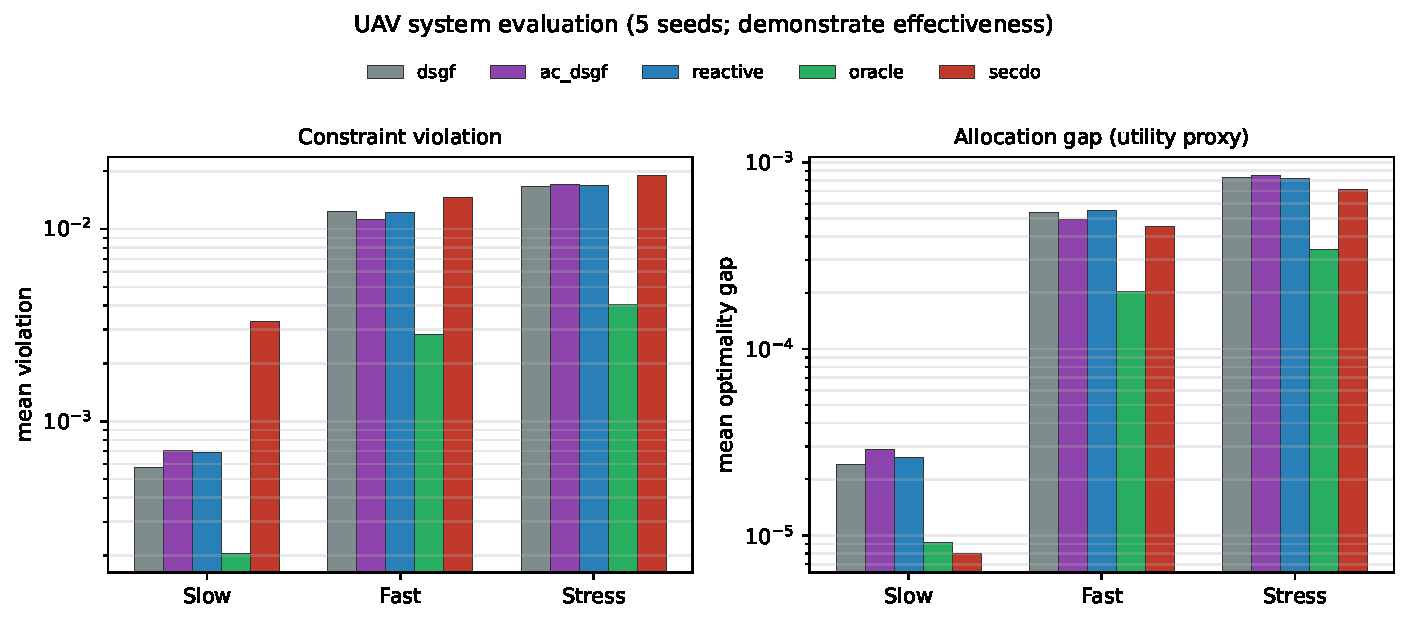
\includegraphics[width=\linewidth]{figures/fig5_uav.pdf}
\caption{Optimality--safety trade-off under dynamic constraints (UAV, 5 seeds).
SECDO achieves a favorable gap--violation trade-off relative to conservative reactive baselines.
Oracle uses future $c_{t+1}$ (informational upper bound).}
\label{fig:uav}
\end{figure}
Fig.~\ref{fig:uav}: SECDO reduces optimality gap by exploiting constraint evolution, at a moderate violation cost versus reactive methods---the expected anticipatory vs.\ conservative trade-off.

\subsection{Ablation}
\begin{table}[t]
\centering
\caption{Ablation on Fast UAV regret and crash-window cumulative-violation rise.}
\label{tab:ablation}
\begin{tabular}{lcc}
\toprule
Variant & Fast $\mathrm{Reg}_T$ & Crash window rise \\
\midrule
Full SECDO & 0.044 & 0.185 \\
A1/A2 (no anticipation) & 0.052 (+18\%) & 0.142 \\
A3 ($\alpha\equiv 1$) & 0.043 & 0.559 ($\times$3) \\
\bottomrule
\end{tabular}
\end{table}
Table~\ref{tab:ablation}: removing anticipation increases Fast regret by $\sim\!18\%$.
Adaptive $\alpha$ mainly improves robustness rather than nominal performance:
when predictions are accurate, $\alpha\equiv 1$ is nearly unchanged; under failure it prevents error amplification (Corollary~\ref{cor:4}).
